\documentclass{article}

\usepackage{mathtools,amsfonts}
\usepackage{enumerate}
\usepackage{fullpage}
\usepackage{fancyvrb}
\usepackage{hyperref}
\usepackage{amsthm}
\usepackage{graphicx}

\newtheorem*{lemma}{Lemma}


\begin{document}
\thispagestyle{empty}

\begin{center}
  \textbf{\Large Advanced February Monthly Assignment Solutions}
\end{center}

\vspace{12pt}

\begin{enumerate}[1.]

\vspace{24pt}
\item % Danielle/Taariq
{\itshape Let $c$ and $d$ be positive divisors of a natural number $n$ such that $c > d$. Prove that $$c > d + \frac{d^2}{n}.$$}

Let $n = kc = md$. The inequality that we want to prove is then equivalent to
\[
	\frac{n}{k} > \frac{n}{m} + \frac{\frac{n^2}{m^2}}{n} \iff \frac{1}{k} > \frac{1}{m} + \frac{1}{m^2} \iff m^2 > mk + k.
\]
Since $c > d$, we have that $k < m$, and so $k \leq m - 1$, and so we have that
\[
	mk + k = k(m + 1) \leq (m - 1)(m + 1) = m^2 - 1 < m^2
\]
which proves the desired result.


\vspace{24pt}
\item % Ireland 2018 Q9
{\itshape Suppose $a,b,c > 0$ and $\sqrt{a-b} +\sqrt{a-c} > \sqrt{b+c}$. Prove that $a > \dfrac{3}{4} (b+c)$.}

Suppose that $a \leq \dfrac{3}{4} (b + c)$. We will show that $\sqrt{a-b} +\sqrt{a-c} \leq \sqrt{b+c}$. Since $a \leq \dfrac{3}{4} (b + c)$, we have that
\[
	\sqrt{a-b} +\sqrt{a-c} \leq \sqrt{\frac{3}{4}(b + c) - b} + \sqrt{\frac{3}{4}(b + c) - c} = \frac{1}{2} \left(\sqrt{3c - b} + \sqrt{3b - c}\right).
\]

We thus wish to show that
\[
	\dfrac{1}{2} \left(\sqrt{3c - b} + \sqrt{3b - c}\right)  \leq \sqrt{b + c}.
\]
By squaring both sides, this is equivalent to
\[
	(3c - b) + (3b - c) + 2\sqrt{(3c - b)(3b - c)}  \leq 4(b + c).
\]
We move the terms not under the square-root to the right hand side, divide by $2$, and square again to obtain
\[
	(3c - b)(3b - c) \leq (b + c)^2.
\]
Expanding each side of this inequality leads us to want to prove that
\[
	10bc - 3b^2 - 3c^2 \leq b^2 + 2bc + c^2
\]
which is equivalent to
\[
	4(b - c)^2 \geq 0
\]
and so we are done.


\vspace{24pt}
\item % NH-2006-1
{\itshape Let $ABCD$ be a square.
Points $P$ and $Q$ lie on the segments $AD$ and $DC$ such that $\angle PBQ = 45^\circ$.
Prove that $BP$ bisects $\angle APQ$ and $BQ$ bisects $\angle CQP$.}

\begin{figure}[!ht]
	\centering
	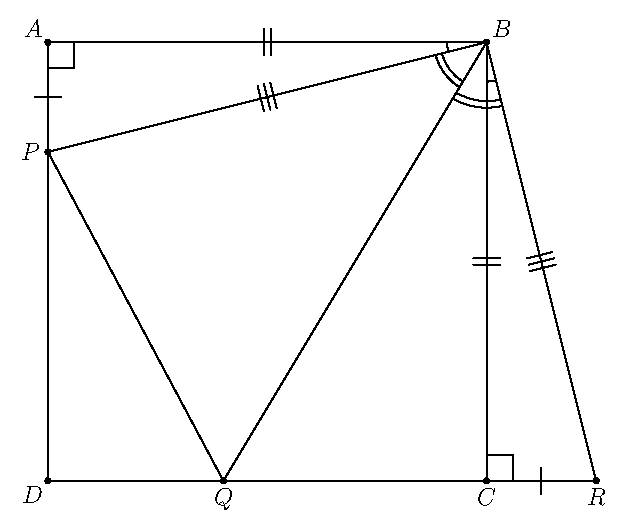
\includegraphics{advanced_february_problem3.eps}
	\caption{Problem 3}
\end{figure}

Let $R$ be a point on $DC$ extended such that $CR = AP$. Then in triangles $BAP$ and $BCR$, we have that $AP = CR$, $BA = BC$, and $\angle BAP = \angle BCR = 90^\circ$. It follows that $\triangle BAP \cong \triangle BCR$, and so in particular we have that $BP = BR$ and $\angle ABP = \angle CBR$.

We note this this implies that $\angle QBR = \angle QBC + \angle CBR = \angle QBC + \angle ABP = 90^\circ - \angle PBQ = 45^\circ = \angle QBP$.

In triangles $QBP$ and $QBR$, we thus have that $QB$ is common, $BP = BR$, and $\angle QBP = \angle QBR$. Thus $\triangle QBP \cong \triangle QBR$, and so $\angle RQB = \angle PQB$, as we wished to show. A similar argument shows that $\angle QPB = \angle APB$.


\vspace{24pt}
\item % French Number Theory Training Assignment
{\itshape Let $n$ be a positive integer. Show that there is a positive integer $m$ such that $\varphi(m) = n!$, where $\varphi$ denotes the Euler phi function.}

Call a natural number $n$ \emph{sufficiently factorial-like} if whenever $p_1, p_2, \dots, p_k$ are distinct prime factors of $n$, we have that $(p_1 - 1)(p_2 - 1) \dotsb (p_k - 1) \mid n$. Note that $n!$ is always sufficiently factorial-like.

We will prove the following result, of which the current problem is a special case:
\begin{lemma}
	Suppose that $n$ is sufficiently factorial-like. Then there is a natural number $m$ such that $\varphi(m) = n$, and such that if $p$ is any prime that divides $m$, then $p$ divides $n$.
\end{lemma}
\begin{proof}
	We proceed by strong induction. We note that $1$ is sufficiently factorial-like, and that $\phi(1) = 1$.

	Suppose that $n$ is sufficiently factorial-like, and that for all sufficiently factorial-like natural numbers $a < n$, there is a natural number $b$ such that $\varphi(b) = a$ where all of the prime divisors of $b$ are also prime divisors of $a$. We will construct a natural number $m$ such that $\varphi(m) = n$ and such that all of the prime divisors of $m$ are also prime divisors of $n$.

	Let $p$ be the largest prime number that divides $n$, and let $p^k$ be the largest power of $p$ that divides $n$. Let $a = \dfrac{n}{p^k(p - 1)}$. Clearly $a < n$. We claim that $a$ is sufficiently factorial-like.

	Suppose that $p_1, p_2, \dots, p_k$ be distinct prime factors of $a$. Then $p_1, p_2, \dots, p_k, p$ are distinct prime factors of $n$, and so since $n$ is sufficiently factorial-like, we have that
	\[
		(p_1 - 1)(p_2 - 1) \dotsb (p_k - 1)(p - 1) \mid n = p^k(p - 1) a.
	\]
	Since $p$ was the largest prime factor of $n$, we have that $p \geq p_i > p_i - 1$ for each $i$, and so $p$ does not divide $p_i - 1$. It follows that
	\[
		\gcd((p_1 - 1)(p_2 - 1) \dotsb (p_k - 1), p^k) = 1,
	\]
	and so we have that $(p_1 - 1)(p_2 - 1) \dotsb (p_k - 1)$ divides $a$ by Euclid's Lemma. We see that $a$ is indeed sufficiently factorial-like. By the induction hypothesis, there is a natural number $b$ such that $\varphi(b) = a$, and such that all of the prime factors of $b$ are prime factors of $a$. This implies that $p$ is not a prime factor of $b$, and so the numbers $p^{k + 1}$ and $b$ are relatively prime. Let $m = p^{k + 1} b$. Then
	\[
		\varphi(m) = \varphi\left(p^{k + 1} b\right) = \varphi\left(p^{k + 1}\right) \varphi(b) = p^k (p - 1) a = n.
	\]

	Since all of the prime factors of $m$ are also factors of $n$ (they are either $p$, which is a factor of $n$, or a prime factor of $b$, thus a factor of $a$, thus a factor of $n$) we see that the desired result holds true for $n$ as well. By the principle of strong mathematical induction, we have that the lemma is true for all sufficiently factorial-like natural numbers $n$.
\end{proof}


\vspace{24pt}
\item % China North MO 2020 Advanced Level P1
{\itshape Define the function $f(x) = x^2 + \sin(x)$ (where $x$ is in radians in this context). Furthermore, let $\{a_n\}$ be a sequence with $a_n \in \mathbb{R}^+$ for all $n \in \mathbb{N}$. Let $a_1 = 1$, and $f(a_n) = a_{n - 1}$ for $n \ge 2$. Prove that there exists $n \in \mathbb{N}$ such that 
$$\sum_{k = 1}^n a_i > 2021.$$}

We will show by induction on $n$ that $a_n \geq \dfrac{1}{n}$ for all natural numbers $n$. This is true for $n = 1$. Suppose that $a_n \geq \dfrac{1}{n}$ for some $n$. Then we have that
\[
	a_{n + 1}^2 + a_{n + 1} \geq a_{n + 1}^2 + \sin(a_{n + 1}) = f(a_{n + 1}) = a_n \geq \dfrac{1}{n},
\]
using the well-known fact that $\sin(x) \leq x$ for all positive real numbers $x$. To show that this implies that $a_{n + 1} \geq \dfrac{1}{n + 1}$, we note that the function $x \mapsto x^2 + x$ is increasing over the positive real numbers, and so it is sufficient to show that
\[
	\left(\frac{1}{n + 1}\right)^2 + \frac{1}{n + 1} \leq \dfrac{1}{n}.
\]
But this is equivalent to
\[
	n + n(n + 1) \leq (n + 1)^2
\]
which in turn simplifies to $0 \leq 1$.

We recall that the sum
\[
	\sum_{k=1}^{n} \frac{1}{k}
\]
can be made arbitrarily large by taking $n$ large enough. It follows that the same is true of the sum
\[
	\sum_{k=1}^{n} a_k.	
\]


\vspace{24pt}
\item % Ukraine 2016-2017 p54 Q10
{\itshape Consider a triangle $ABC$ with points $M$ and $N$ on $BC$ and $AB$ respectively such that $AM \perp BC$ and $CN \perp AB$, and let $AC$ and $MN$ intersect at $Y$.
It is given $X$ is a point inside acute-angled triangle $ABC$ such that $MBNX$ is a parallelogram.
Prove that the angle bisectors of $\angle MXN$ and $\angle MYC$ are perpendicular.}

\begin{figure}[!ht]
	\centering
	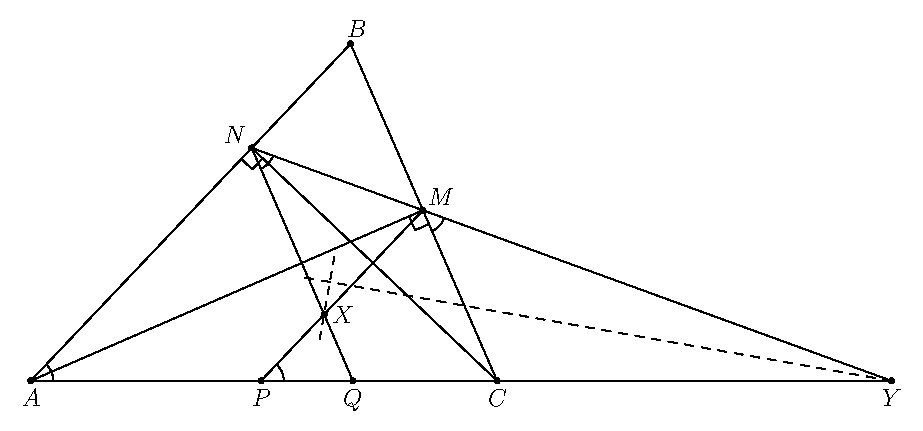
\includegraphics{advanced_february_problem6.eps}
	\caption{Problem 6}\label{fig:q6part1}
\end{figure}

Let $P$ and $Q$ be the points of intersection of the lines $MX$ and $NX$ with the line $AC$ respectively. Consider the arrangement of points in Figure \ref{fig:q6part1}. We will show that $\angle QPM = \angle QNM$.

Since $\angle ANC = \angle AMC = 90^\circ$, we have that the points $A$, $N$, $M$, and $C$ are concyclic, implying that $\angle CAN = \angle CMY$. Since $MX \parallel BA$, we have that $\angle QPM = \angle CAN$, and since $NX \parallel BC$, we have that $\angle QNM = \angle CMY$. Hence $\angle QPM = \angle QNM$, as claimed.

\begin{figure}[!hb]
	\centering
	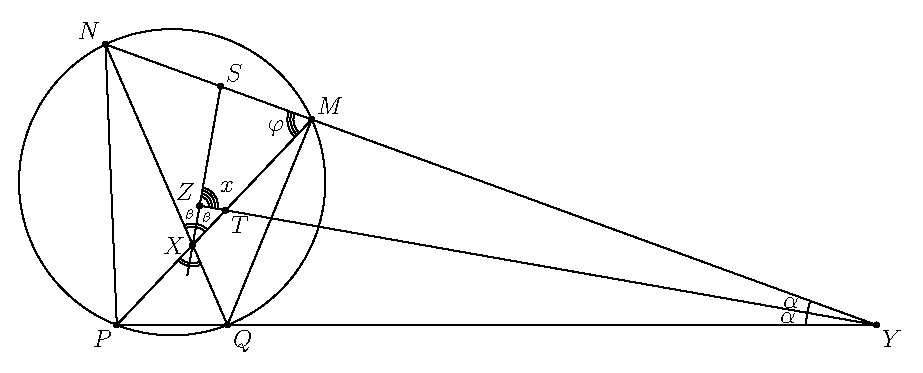
\includegraphics{advanced_february_problem6_part2.eps}
	\caption{Problem 6}\label{fig:q6part2}
\end{figure}

Let $Z$ be the intersection of the bisectors of angles $\angle MXN$ and $\angle MYC$. Let $T$ be intersection of $PM$ and $YZ$ (extended), and let $S$ be the intersection of $NM$ and $XZ$ (extended). Let $x$, $\alpha$, $\beta$, and $\varphi$ be the angled marked as such in Figure \ref{fig:q6part2}.

Then the angles of the triangle $XZT$ are as follows: $\angle TXZ = \beta$, $\angle XZT = 180^\circ - x$, and $\angle XTZ = \varphi - \alpha$ by the exterior angle theorem in triangle $TMY$. These angles sum to $180^\circ$, and so we have that $\beta + 180^\circ - x + \varphi - \alpha = 180^\circ$, or equivalently that $x = \beta + \varphi - \alpha$.

Finally, we prove that $\beta + \varphi - \alpha = 90^\circ$. The angles in triangle $MXN$ sum to $180^\circ$, and so we have that $\angle QNM = \angle XNM = 180^\circ - 2\beta - \varphi$. We also know that $\angle QPM = \angle YPM = \varphi - 2\alpha$ by the exterior angle theorem in triangle $PMY$. We proved earlier that $\angle QPM = \angle QNM$. This implies that $180^\circ - 2\beta - \varphi = \varphi - 2\alpha$, and so $\beta + \varphi - \alpha = 90^\circ$, as desired.


\end{enumerate}

\end{document}
